

\tikzset{every picture/.style={line width=0.75pt}} %set default line width to 0.75pt        

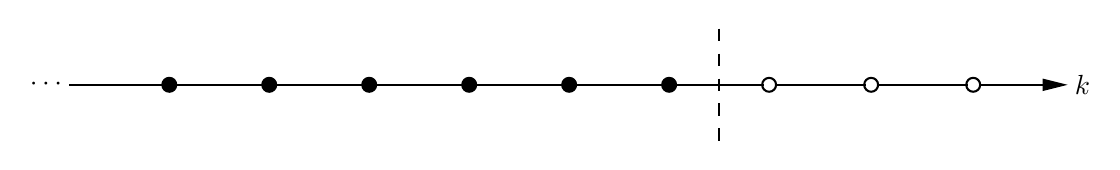
\begin{tikzpicture}[x=0.75pt,y=0.75pt,yscale=-1,xscale=1]
%uncomment if require: \path (0,300); %set diagram left start at 0, and has height of 300

%Straight Lines [id:da389985056516742] 
\draw    (100,102) -- (148.17,102) ;
\draw [shift={(148.17,102)}, rotate = 0] [color={rgb, 255:red, 0; green, 0; blue, 0 }  ][fill={rgb, 255:red, 0; green, 0; blue, 0 }  ][line width=0.75]      (0, 0) circle [x radius= 3.35, y radius= 3.35]   ;
%Straight Lines [id:da8735536812464386] 
\draw    (148.17,102) -- (196.33,102) ;
\draw [shift={(196.33,102)}, rotate = 0] [color={rgb, 255:red, 0; green, 0; blue, 0 }  ][fill={rgb, 255:red, 0; green, 0; blue, 0 }  ][line width=0.75]      (0, 0) circle [x radius= 3.35, y radius= 3.35]   ;
%Straight Lines [id:da7221208832553236] 
\draw    (196.33,102) -- (244.5,102) ;
\draw [shift={(244.5,102)}, rotate = 360] [color={rgb, 255:red, 0; green, 0; blue, 0 }  ][fill={rgb, 255:red, 0; green, 0; blue, 0 }  ][line width=0.75]      (0, 0) circle [x radius= 3.35, y radius= 3.35]   ;
%Straight Lines [id:da22657899441580232] 
\draw    (244.5,102) -- (292.67,102) ;
\draw [shift={(292.67,102)}, rotate = 0] [color={rgb, 255:red, 0; green, 0; blue, 0 }  ][fill={rgb, 255:red, 0; green, 0; blue, 0 }  ][line width=0.75]      (0, 0) circle [x radius= 3.35, y radius= 3.35]   ;
%Straight Lines [id:da055761283547104634] 
\draw    (292.67,102) -- (340.83,102) ;
\draw [shift={(340.83,102)}, rotate = 0] [color={rgb, 255:red, 0; green, 0; blue, 0 }  ][fill={rgb, 255:red, 0; green, 0; blue, 0 }  ][line width=0.75]      (0, 0) circle [x radius= 3.35, y radius= 3.35]   ;
%Straight Lines [id:da9070988727925184] 
\draw    (340.83,102) -- (389,102) ;
\draw [shift={(389,102)}, rotate = 0] [color={rgb, 255:red, 0; green, 0; blue, 0 }  ][fill={rgb, 255:red, 0; green, 0; blue, 0 }  ][line width=0.75]      (0, 0) circle [x radius= 3.35, y radius= 3.35]   ;
%Straight Lines [id:da57324706717669] 
\draw    (538.5,102) -- (579,102) ;
\draw [shift={(581,102)}, rotate = 180] [fill={rgb, 255:red, 0; green, 0; blue, 0 }  ][line width=0.08]  [draw opacity=0] (12,-3) -- (0,0) -- (12,3) -- cycle    ;
%Straight Lines [id:da567630885526011] 
\draw    (440.17,102) -- (483.98,102) ;
\draw [shift={(486.33,102)}, rotate = 0] [color={rgb, 255:red, 0; green, 0; blue, 0 }  ][line width=0.75]      (0, 0) circle [x radius= 3.35, y radius= 3.35]   ;
%Straight Lines [id:da8582364164149097] 
\draw [fill={rgb, 255:red, 255; green, 255; blue, 255 }  ,fill opacity=1 ]   (389,102) -- (434.82,102) ;
\draw [shift={(437.17,102)}, rotate = 0] [color={rgb, 255:red, 0; green, 0; blue, 0 }  ][line width=0.75]      (0, 0) circle [x radius= 3.35, y radius= 3.35]   ;
%Straight Lines [id:da039926120326623904] 
\draw  [dash pattern={on 4.5pt off 4.5pt}]  (413.08,74.98) -- (413.08,129.02) ;
%Straight Lines [id:da05138302077418411] 
\draw    (489.33,102) -- (533.15,102) ;
\draw [shift={(535.5,102)}, rotate = 0] [color={rgb, 255:red, 0; green, 0; blue, 0 }  ][line width=0.75]      (0, 0) circle [x radius= 3.35, y radius= 3.35]   ;

% Text Node
\draw (98,102) node [anchor=east] [inner sep=0.75pt]   [align=left] {$\displaystyle \cdots $};
% Text Node
\draw (583,102) node [anchor=west] [inner sep=0.75pt]    {$k$};


\end{tikzpicture}
